\chapter{Coleções}

    Tendo em vista a máxima rapidez no acesso a dados por parte dos utilizadores do sistema, deve ser dada relevância à forma como os registos são armazenados, visto que estes devem poder ser consultados em tempo constante.

    A forma mais fácil de garantir isto é obviamente através da utilização de \textit{Map's,} contudo em alguns casos a sua utilização não é necessária, podendo mesmo ser utilizadas listas.

    Ainda dentro das coleções, podemos adotar uma estratégia de associação ou composição, e tendo em conta que a composição é em certa medida mais segura, dado que implica a criação de cópias, optámos por seguir essa abordagem, mesmo sabendo que por outro lado está a ser desperdiçada memória que possa vir a ser útil no futuro.

    \section{Utilizador}

    \begin{figure}[hb!]
        \centering
        \vspace{-10pt}
        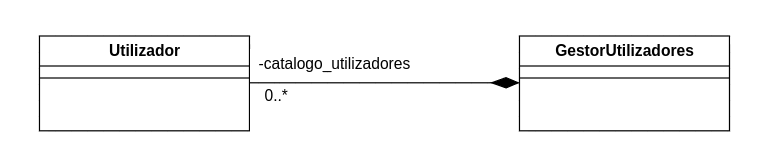
\includegraphics[width=0.7\textwidth]{imagens/5.png}
        \caption*{Figura 5. Coleção de Utilizadores}
    \end{figure}
    \vspace{8pt}

    A coleção de utilizadores é o único caso em que não é utilizado um \textit{Map,} mas sim uma lista, pois tendo em conta que os utilizadores são identificados por um número, podemos associar esse mesmo número ao índice da sua possui na lista, garantido assim o acesso direto.

    \section{Encomenda}

    \begin{figure}[hb!]
        \centering
        \vspace{-5pt}
        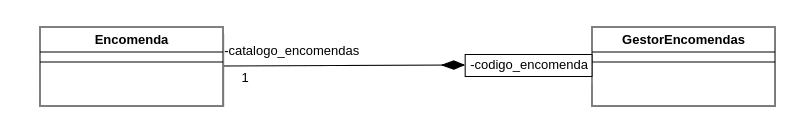
\includegraphics[width=0.7\textwidth]{imagens/14.png}
        \caption*{Figura 6. Coleção de Encomendas}
        \vspace{5pt}
    \end{figure}
    \vspace{8pt}

    Tal como os utilizadores, as encomendas também são identificadas por um número, portanto seria admissível utilizar a mesma estratégia, contudo optámos por utilizar um \textit{Map} sem nenhuma razão em específico.
    
    \section{Transportadora}

    \begin{figure}[hb!]
        \centering
        \vspace{-5pt}
        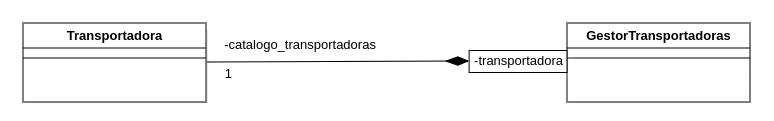
\includegraphics[width=0.7\textwidth]{imagens/13.png}
        \caption*{Figura 7. Coleção de Transportadoras}
    \end{figure}
    \vspace{8pt}

    Ao contrário dos casos anteriores, em que o objeto era identificado univocamente por um inteiro, neste caso uma transportadora tem associada a si um nome que a caracteriza, como tal cada objeto desta classe é guardado num \textit{Map} cuja chave é o \textit{hashCode} do nome da transportadora.

    \section{Artigo}

    \begin{figure}[hb!]
        \centering
        \vspace{-15pt}
        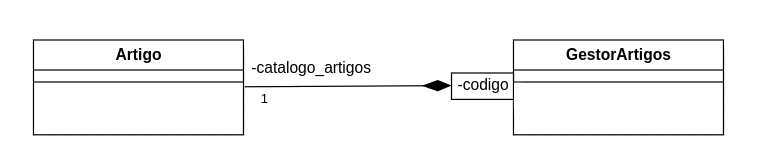
\includegraphics[width=0.7\textwidth]{imagens/4.png}
        \caption*{Figura 8. Coleção de Artigos}
    \end{figure}
    \vspace{8pt}

    A exemplo de uma transportadora, um artigo é caracterizado por um código alfanumérico, ou seja, uma \textit{String}, portanto a coleção implementada é a mesma.

    \section{Fatura}

    \begin{figure}[hb!]
        \centering
        \vspace{-10pt}
        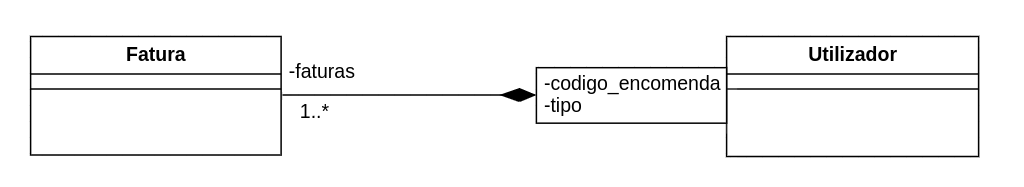
\includegraphics[width=0.7\textwidth]{imagens/12.png}
        \caption*{Figura 9. Coleção de Faturas}
    \end{figure}
    \vspace{8pt}

    A criação de uma classe fatura a princípio não parece óbvia, contudo se queremos saber o dinheiro ganho/gasto por um determinado utilizador, convém ter esses valores previamente calculados a fim de responder rapidamente às interrogações estatísticas.

    Como tal, quando uma encomenda é finalizada, o utilizador recebe uma fatura por cada artigo que esta possui, e assim, à medida que as faturas são inserida no \textit{Map,} apenas uma é preservada, sendo que o preço desta corresponde ao somatório do preço das restantes.

    Além disso, há que ter em atenção que numa encomenda existem dois lados, o de quem compra, e o de quem vende, como tal a chave de uma entrada do \textit{Map} não é somente o código da encomenda, mas sim uma combinação entre este e o tipo, que indica se um determinado utilizador age como vendedor ou comprador perante uma encomenda, podendo inclusive agir nos dois papéis em simultâneo.